\Aufgabe{Objektkarten Memory}{
    \doppelseite{0.4}{0.45}{t}{
        \begin{itemize}
            \item Erstelle auf einem Blatt eine Objektkarte der Klasse Person zu dir selbst. $\rightarrow$ \emphColA{3x falten}
            \item Gib deine Objektkarte bei der Lehrkraft ab. $\rightarrow$ Objektkarten werden gemischt.
            \item Ziehe eine Objektkarte und versuche, das zugehörige Objekt zu finden.
            \begin{itemize}
                \item Frage deine:n Gegenüber dafür, ob die Attributwerte auf deiner gezogenen Karte auf sie/ihn zutreffen.
                \item Ihr dürft euch nicht gegenseitig die Objektkarten zeigen!
                \item Wer gefunden wurde, gibt seine aktuelle Objektkarte weiter und setzt sich.
                \item Der/Die Finder:in sammelt alle gefundenen Objekte.
            \end{itemize}
        \end{itemize}
    }{
        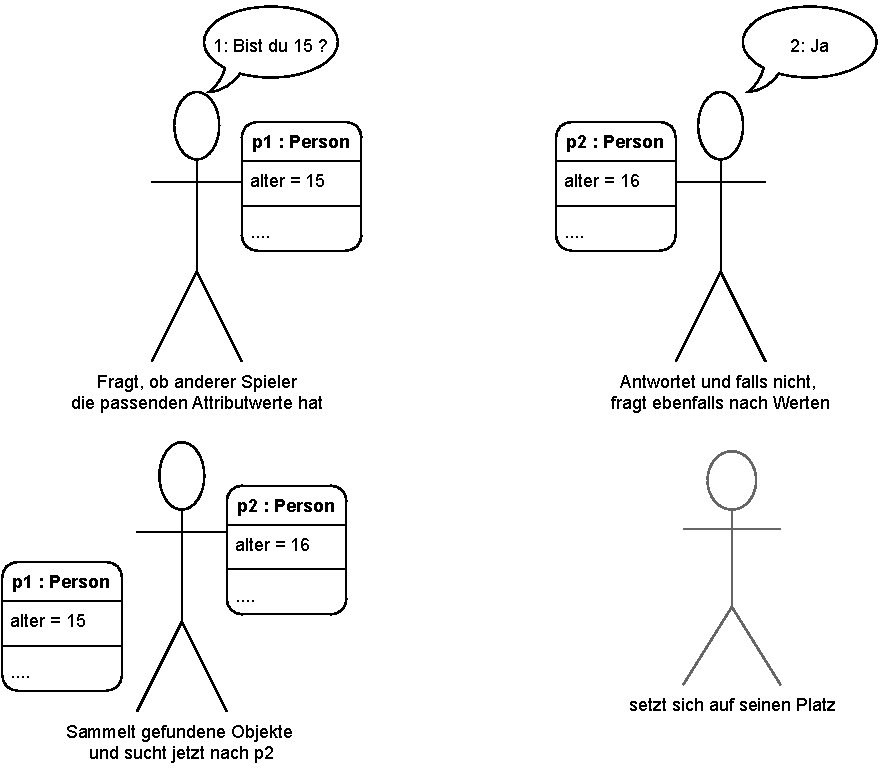
\includegraphics[width=\linewidth]{_Aufgaben/img/A00_Diagramm.pdf} 
    }
}

